

\tikzset{every picture/.style={line width=0.75pt}} %set default line width to 0.75pt        

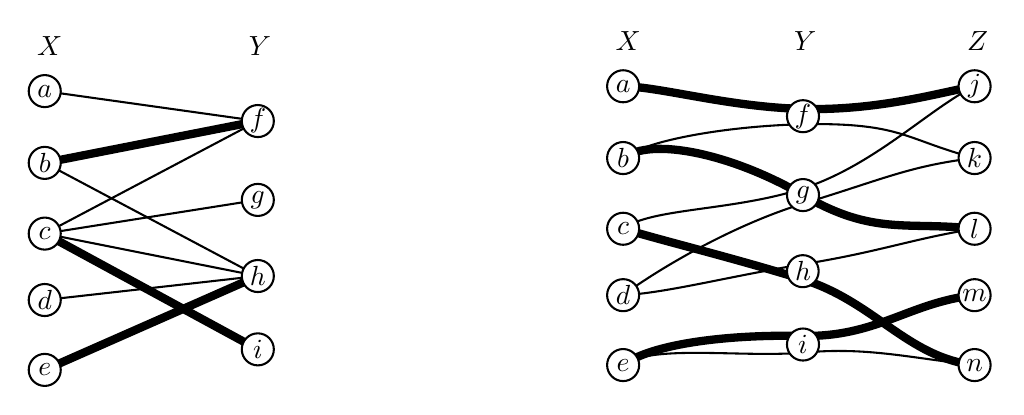
\begin{tikzpicture}[x=0.5pt,y=0.5pt,yscale=-1,xscale=1]
%uncomment if require: \path (0,292); %set diagram left start at 0, and has height of 292

%Curve Lines [id:da4241903757380898] 
\draw [line width=3]    (456.68,55.59) .. controls (484,56) and (534.03,70.9) .. (588,72) .. controls (641.97,73.1) and (686,60) .. (710.68,55.59) ;
%Curve Lines [id:da8255907428390687] 
\draw    (456.68,107.47) .. controls (477.18,92.09) and (551.03,81.9) .. (605,83) .. controls (658.97,84.1) and (664,95) .. (710.68,107.47) ;
%Curve Lines [id:da344500096054706] 
\draw    (456.68,158.57) .. controls (477.18,143.2) and (537,146) .. (588,129) .. controls (639,112) and (679,71) .. (710.68,55.59) ;
%Curve Lines [id:da11085604778848868] 
\draw    (456.68,206.57) .. controls (488,205) and (533,193) .. (588,184) .. controls (643,175) and (665,166) .. (710.68,158.57) ;
%Curve Lines [id:da7960793701320955] 
\draw [line width=3]    (456.68,257.08) .. controls (477.18,241.7) and (532.03,234.9) .. (586,236) .. controls (639.97,237.1) and (663,212) .. (710.68,206.57) ;
%Curve Lines [id:da9523105239538149] 
\draw    (456.68,257.08) .. controls (477.18,241.7) and (543,252) .. (588,248) .. controls (633,244) and (662,251.61) .. (710.68,257.08) ;
%Curve Lines [id:da7884208773008994] 
\draw [line width=3]    (456.68,107.47) .. controls (477.18,92.09) and (535.33,104.46) .. (586.67,134.23) .. controls (638,164) and (662,153.1) .. (710.68,158.57) ;
%Curve Lines [id:da943679960760185] 
\draw    (456.68,206.57) .. controls (477.18,191.2) and (532,157) .. (588,140) .. controls (644,123) and (664,113) .. (710.68,107.47) ;
%Curve Lines [id:da6807255577581136] 
\draw [line width=3]    (456.68,158.57) .. controls (488,168) and (534,179) .. (586,195) .. controls (638,211) and (662,251.61) .. (710.68,257.08) ;
%Straight Lines [id:da5756546325370752] 
\draw [line width=3]    (192.67,80.73) -- (38.68,110.97) ;
%Straight Lines [id:da9211662025642174] 
\draw    (38.68,59.09) -- (192.67,80.73) ;
%Straight Lines [id:da06434668113779485] 
\draw    (192.67,80.73) -- (38.68,162.07) ;
%Straight Lines [id:da4406012177704377] 
\draw    (192.67,192.73) -- (38.68,162.07) ;
%Straight Lines [id:da3723168518652895] 
\draw [line width=3]    (192.67,245.73) -- (38.68,162.07) ;
%Straight Lines [id:da746260912418035] 
\draw    (192.67,137.73) -- (38.68,162.07) ;
%Straight Lines [id:da9456704199726969] 
\draw    (192.67,192.73) -- (38.68,210.07) ;
%Straight Lines [id:da45949818054633906] 
\draw [line width=3]    (192.67,192.73) -- (38.68,260.58) ;
%Straight Lines [id:da9256706423252938] 
\draw    (192.67,192.73) -- (38.68,110.97) ;
%Shape: Ellipse [id:dp2702263199738577] 
\draw  [fill={rgb, 255:red, 255; green, 255; blue, 255 }  ,fill opacity=1 ] (27.1,260.58) .. controls (27.1,254.18) and (32.29,249) .. (38.68,249) .. controls (45.08,249) and (50.26,254.18) .. (50.26,260.58) .. controls (50.26,266.97) and (45.08,272.16) .. (38.68,272.16) .. controls (32.29,272.16) and (27.1,266.97) .. (27.1,260.58) -- cycle ;
%Shape: Ellipse [id:dp19077153467526664] 
\draw  [fill={rgb, 255:red, 255; green, 255; blue, 255 }  ,fill opacity=1 ] (27.1,110.97) .. controls (27.1,104.57) and (32.29,99.39) .. (38.68,99.39) .. controls (45.08,99.39) and (50.26,104.57) .. (50.26,110.97) .. controls (50.26,117.36) and (45.08,122.55) .. (38.68,122.55) .. controls (32.29,122.55) and (27.1,117.36) .. (27.1,110.97) -- cycle ;
%Shape: Ellipse [id:dp5053674258722656] 
\draw  [fill={rgb, 255:red, 255; green, 255; blue, 255 }  ,fill opacity=1 ] (27.1,162.07) .. controls (27.1,155.67) and (32.29,150.49) .. (38.68,150.49) .. controls (45.08,150.49) and (50.26,155.67) .. (50.26,162.07) .. controls (50.26,168.46) and (45.08,173.65) .. (38.68,173.65) .. controls (32.29,173.65) and (27.1,168.46) .. (27.1,162.07) -- cycle ;
%Shape: Ellipse [id:dp6864039160007132] 
\draw  [fill={rgb, 255:red, 255; green, 255; blue, 255 }  ,fill opacity=1 ] (27.1,210.07) .. controls (27.1,203.68) and (32.29,198.49) .. (38.68,198.49) .. controls (45.08,198.49) and (50.26,203.68) .. (50.26,210.07) .. controls (50.26,216.47) and (45.08,221.65) .. (38.68,221.65) .. controls (32.29,221.65) and (27.1,216.47) .. (27.1,210.07) -- cycle ;
%Shape: Ellipse [id:dp6314696709643118] 
\draw  [fill={rgb, 255:red, 255; green, 255; blue, 255 }  ,fill opacity=1 ] (27.1,59.09) .. controls (27.1,52.7) and (32.29,47.51) .. (38.68,47.51) .. controls (45.08,47.51) and (50.26,52.7) .. (50.26,59.09) .. controls (50.26,65.49) and (45.08,70.67) .. (38.68,70.67) .. controls (32.29,70.67) and (27.1,65.49) .. (27.1,59.09) -- cycle ;
%Shape: Ellipse [id:dp5657112261222568] 
\draw  [fill={rgb, 255:red, 255; green, 255; blue, 255 }  ,fill opacity=1 ] (181.09,80.73) .. controls (181.09,74.33) and (186.27,69.15) .. (192.67,69.15) .. controls (199.06,69.15) and (204.25,74.33) .. (204.25,80.73) .. controls (204.25,87.13) and (199.06,92.31) .. (192.67,92.31) .. controls (186.27,92.31) and (181.09,87.13) .. (181.09,80.73) -- cycle ;
%Shape: Ellipse [id:dp46976961266650885] 
\draw  [fill={rgb, 255:red, 255; green, 255; blue, 255 }  ,fill opacity=1 ] (181.09,137.73) .. controls (181.09,131.33) and (186.27,126.15) .. (192.67,126.15) .. controls (199.06,126.15) and (204.25,131.33) .. (204.25,137.73) .. controls (204.25,144.13) and (199.06,149.31) .. (192.67,149.31) .. controls (186.27,149.31) and (181.09,144.13) .. (181.09,137.73) -- cycle ;
%Shape: Ellipse [id:dp8081371923026808] 
\draw  [fill={rgb, 255:red, 255; green, 255; blue, 255 }  ,fill opacity=1 ] (181.09,192.73) .. controls (181.09,186.33) and (186.27,181.15) .. (192.67,181.15) .. controls (199.06,181.15) and (204.25,186.33) .. (204.25,192.73) .. controls (204.25,199.13) and (199.06,204.31) .. (192.67,204.31) .. controls (186.27,204.31) and (181.09,199.13) .. (181.09,192.73) -- cycle ;
%Shape: Ellipse [id:dp9014935828955908] 
\draw  [fill={rgb, 255:red, 255; green, 255; blue, 255 }  ,fill opacity=1 ] (181.09,245.73) .. controls (181.09,239.33) and (186.27,234.15) .. (192.67,234.15) .. controls (199.06,234.15) and (204.25,239.33) .. (204.25,245.73) .. controls (204.25,252.13) and (199.06,257.31) .. (192.67,257.31) .. controls (186.27,257.31) and (181.09,252.13) .. (181.09,245.73) -- cycle ;
%Shape: Ellipse [id:dp6377243000988755] 
\draw  [fill={rgb, 255:red, 255; green, 255; blue, 255 }  ,fill opacity=1 ] (445.1,257.08) .. controls (445.1,250.68) and (450.29,245.5) .. (456.68,245.5) .. controls (463.08,245.5) and (468.26,250.68) .. (468.26,257.08) .. controls (468.26,263.47) and (463.08,268.66) .. (456.68,268.66) .. controls (450.29,268.66) and (445.1,263.47) .. (445.1,257.08) -- cycle ;
%Shape: Ellipse [id:dp8875585136863995] 
\draw  [fill={rgb, 255:red, 255; green, 255; blue, 255 }  ,fill opacity=1 ] (445.1,107.47) .. controls (445.1,101.07) and (450.29,95.89) .. (456.68,95.89) .. controls (463.08,95.89) and (468.26,101.07) .. (468.26,107.47) .. controls (468.26,113.86) and (463.08,119.05) .. (456.68,119.05) .. controls (450.29,119.05) and (445.1,113.86) .. (445.1,107.47) -- cycle ;
%Shape: Ellipse [id:dp34090468871105073] 
\draw  [fill={rgb, 255:red, 255; green, 255; blue, 255 }  ,fill opacity=1 ] (445.1,158.57) .. controls (445.1,152.17) and (450.29,146.99) .. (456.68,146.99) .. controls (463.08,146.99) and (468.26,152.17) .. (468.26,158.57) .. controls (468.26,164.96) and (463.08,170.15) .. (456.68,170.15) .. controls (450.29,170.15) and (445.1,164.96) .. (445.1,158.57) -- cycle ;
%Shape: Ellipse [id:dp5749980491800895] 
\draw  [fill={rgb, 255:red, 255; green, 255; blue, 255 }  ,fill opacity=1 ] (445.1,206.57) .. controls (445.1,200.18) and (450.29,194.99) .. (456.68,194.99) .. controls (463.08,194.99) and (468.26,200.18) .. (468.26,206.57) .. controls (468.26,212.97) and (463.08,218.15) .. (456.68,218.15) .. controls (450.29,218.15) and (445.1,212.97) .. (445.1,206.57) -- cycle ;
%Shape: Ellipse [id:dp45930415406985825] 
\draw  [fill={rgb, 255:red, 255; green, 255; blue, 255 }  ,fill opacity=1 ] (445.1,55.59) .. controls (445.1,49.2) and (450.29,44.01) .. (456.68,44.01) .. controls (463.08,44.01) and (468.26,49.2) .. (468.26,55.59) .. controls (468.26,61.99) and (463.08,67.17) .. (456.68,67.17) .. controls (450.29,67.17) and (445.1,61.99) .. (445.1,55.59) -- cycle ;
%Shape: Ellipse [id:dp19109391131087505] 
\draw  [fill={rgb, 255:red, 255; green, 255; blue, 255 }  ,fill opacity=1 ] (699.1,257.08) .. controls (699.1,250.68) and (704.29,245.5) .. (710.68,245.5) .. controls (717.08,245.5) and (722.26,250.68) .. (722.26,257.08) .. controls (722.26,263.47) and (717.08,268.66) .. (710.68,268.66) .. controls (704.29,268.66) and (699.1,263.47) .. (699.1,257.08) -- cycle ;
%Shape: Ellipse [id:dp6608460236903059] 
\draw  [fill={rgb, 255:red, 255; green, 255; blue, 255 }  ,fill opacity=1 ] (699.1,107.47) .. controls (699.1,101.07) and (704.29,95.89) .. (710.68,95.89) .. controls (717.08,95.89) and (722.26,101.07) .. (722.26,107.47) .. controls (722.26,113.86) and (717.08,119.05) .. (710.68,119.05) .. controls (704.29,119.05) and (699.1,113.86) .. (699.1,107.47) -- cycle ;
%Shape: Ellipse [id:dp5555355188552026] 
\draw  [fill={rgb, 255:red, 255; green, 255; blue, 255 }  ,fill opacity=1 ] (699.1,158.57) .. controls (699.1,152.17) and (704.29,146.99) .. (710.68,146.99) .. controls (717.08,146.99) and (722.26,152.17) .. (722.26,158.57) .. controls (722.26,164.96) and (717.08,170.15) .. (710.68,170.15) .. controls (704.29,170.15) and (699.1,164.96) .. (699.1,158.57) -- cycle ;
%Shape: Ellipse [id:dp6338528995548398] 
\draw  [fill={rgb, 255:red, 255; green, 255; blue, 255 }  ,fill opacity=1 ] (699.1,206.57) .. controls (699.1,200.18) and (704.29,194.99) .. (710.68,194.99) .. controls (717.08,194.99) and (722.26,200.18) .. (722.26,206.57) .. controls (722.26,212.97) and (717.08,218.15) .. (710.68,218.15) .. controls (704.29,218.15) and (699.1,212.97) .. (699.1,206.57) -- cycle ;
%Shape: Ellipse [id:dp17174353029329448] 
\draw  [fill={rgb, 255:red, 255; green, 255; blue, 255 }  ,fill opacity=1 ] (699.1,55.59) .. controls (699.1,49.2) and (704.29,44.01) .. (710.68,44.01) .. controls (717.08,44.01) and (722.26,49.2) .. (722.26,55.59) .. controls (722.26,61.99) and (717.08,67.17) .. (710.68,67.17) .. controls (704.29,67.17) and (699.1,61.99) .. (699.1,55.59) -- cycle ;
%Shape: Ellipse [id:dp8143115518987177] 
\draw  [fill={rgb, 255:red, 255; green, 255; blue, 255 }  ,fill opacity=1 ] (575.09,134.23) .. controls (575.09,127.83) and (580.27,122.65) .. (586.67,122.65) .. controls (593.06,122.65) and (598.25,127.83) .. (598.25,134.23) .. controls (598.25,140.63) and (593.06,145.81) .. (586.67,145.81) .. controls (580.27,145.81) and (575.09,140.63) .. (575.09,134.23) -- cycle ;
%Shape: Ellipse [id:dp4472218881975837] 
\draw  [fill={rgb, 255:red, 255; green, 255; blue, 255 }  ,fill opacity=1 ] (575.09,242.23) .. controls (575.09,235.83) and (580.27,230.65) .. (586.67,230.65) .. controls (593.06,230.65) and (598.25,235.83) .. (598.25,242.23) .. controls (598.25,248.63) and (593.06,253.81) .. (586.67,253.81) .. controls (580.27,253.81) and (575.09,248.63) .. (575.09,242.23) -- cycle ;
%Shape: Ellipse [id:dp41243068424191065] 
\draw  [fill={rgb, 255:red, 255; green, 255; blue, 255 }  ,fill opacity=1 ] (575.09,189.23) .. controls (575.09,182.83) and (580.22,177.65) .. (586.54,177.65) .. controls (592.87,177.65) and (598,182.83) .. (598,189.23) .. controls (598,195.63) and (592.87,200.81) .. (586.54,200.81) .. controls (580.22,200.81) and (575.09,195.63) .. (575.09,189.23) -- cycle ;
%Shape: Ellipse [id:dp03176181710264381] 
\draw  [fill={rgb, 255:red, 255; green, 255; blue, 255 }  ,fill opacity=1 ] (575.09,77.23) .. controls (575.09,70.83) and (580.27,65.65) .. (586.67,65.65) .. controls (593.06,65.65) and (598.25,70.83) .. (598.25,77.23) .. controls (598.25,83.63) and (593.06,88.81) .. (586.67,88.81) .. controls (580.27,88.81) and (575.09,83.63) .. (575.09,77.23) -- cycle ;

% Text Node
\draw (38.68,260.58) node   [align=left] {$\displaystyle e$};
% Text Node
\draw (38.68,110.97) node   [align=left] {$\displaystyle b$};
% Text Node
\draw (38.68,162.07) node   [align=left] {$\displaystyle c$};
% Text Node
\draw (38.68,210.07) node   [align=left] {$\displaystyle d$};
% Text Node
\draw (38.68,59.09) node   [align=left] {$\displaystyle a$};
% Text Node
\draw (192.67,80.73) node   [align=left] {$\displaystyle f$};
% Text Node
\draw (192.67,137.73) node   [align=left] {$\displaystyle g$};
% Text Node
\draw (192.67,192.73) node   [align=left] {$\displaystyle h$};
% Text Node
\draw (192.67,245.73) node   [align=left] {$\displaystyle i$};
% Text Node
\draw (31,17.5) node [anchor=north west][inner sep=0.75pt]   [align=left] {$\displaystyle X$};
% Text Node
\draw (184,17.5) node [anchor=north west][inner sep=0.75pt]   [align=left] {$\displaystyle Y$};
% Text Node
\draw (456.68,257.08) node   [align=left] {$\displaystyle e$};
% Text Node
\draw (456.68,107.47) node   [align=left] {$\displaystyle b$};
% Text Node
\draw (456.68,158.57) node   [align=left] {$\displaystyle c$};
% Text Node
\draw (456.68,206.57) node   [align=left] {$\displaystyle d$};
% Text Node
\draw (456.68,55.59) node   [align=left] {$\displaystyle a$};
% Text Node
\draw (586.67,77.23) node   [align=left] {$\displaystyle f$};
% Text Node
\draw (586.67,134.23) node   [align=left] {$\displaystyle g$};
% Text Node
\draw (586.67,189.23) node   [align=left] {$\displaystyle h$};
% Text Node
\draw (586.67,242.23) node   [align=left] {$\displaystyle i$};
% Text Node
\draw (449,14) node [anchor=north west][inner sep=0.75pt]   [align=left] {$\displaystyle X$};
% Text Node
\draw (578,14) node [anchor=north west][inner sep=0.75pt]   [align=left] {$\displaystyle Y$};
% Text Node
\draw (710.68,257.08) node   [align=left] {$\displaystyle n$};
% Text Node
\draw (710.68,107.47) node   [align=left] {$\displaystyle k$};
% Text Node
\draw (710.68,158.57) node   [align=left] {$\displaystyle l$};
% Text Node
\draw (710.68,206.57) node   [align=left] {$\displaystyle m$};
% Text Node
\draw (710.68,55.59) node   [align=left] {$\displaystyle j$};
% Text Node
\draw (703,14) node [anchor=north west][inner sep=0.75pt]   [align=left] {$\displaystyle Z$};


\end{tikzpicture}

